%%%%%%%%%%%%%%%%%%%%%%%%%%%%%%%%%%%%%%%%%
% Friggeri Resume/CV
% XeLaTeX Template
% Version 1.0 (5/5/13)
%
% This template has been downloaded from:
% http://www.LaTeXTemplates.com
%
% Original author:
% Adrien Friggeri (adrien@friggeri.net)
% https://github.com/afriggeri/CV
%
% License:
% CC BY-NC-SA 3.0 (http://creativecommons.org/licenses/by-nc-sa/3.0/)
%
% Important notes:
% This template needs to be compiled with XeLaTeX and the bibliography, if used,
% needs to be compiled with biber rather than bibtex.
%
%%%%%%%%%%%%%%%%%%%%%%%%%%%%%%%%%%%%%%%%%

\documentclass[]{friggeri-cv} % Add 'print' as an option into the square bracket to remove colors from this template for printing

\listfiles

\addbibresource{bibliography_auto.bib} 

\begin{document}

\header{Guillaume}{Lobet}{Assistant Professor - Functional structural modelling of crop systems}


%----------------------------------------------------
%----------------------------------------------------
%	SIDEBAR SECTION
%----------------------------------------------------
%----------------------------------------------------

\thispagestyle{first}

\begin{aside} 
~\vspace{70pt}


\section{Informations}
~
28-12-1984 [33]
~
g.lobet@fz-juelich.de
~
\href{http://www.guillaumelobet.be}{www.guillaumelobet.be}

~

~\rule{\linewidth}{0.5pt}


~
\section{Keywords}
~
Computational modelling
Image analysis
Data analysis
Web technologies
Science communication
Open Science
~

~\rule{\linewidth}{0.5pt}

~
\section{Languages}
~
French {\color{light}\ding{72}\ding{72}\ding{72}\ding{72}\ding{72}}
English (C1/C2) {\color{light}\ding{72}\ding{72}\ding{72}\ding{72}\ding{73}}
Sign language {\color{light}\ding{72}\ding{73}\ding{73}\ding{73}\ding{73}}


~

~\rule{\linewidth}{0.5pt}
~
\textbf{Note:}\\ All my articles, presentations and projects can be viewed at \href{http://www.guillaumelobet.be}{www.guillaumelobet.be}

\end{aside}



%----------------------------------------------------
%	PROFESIONNAL EXPERIENCE SECTION
%----------------------------------------------------
~\vspace{5pt}
\section{Research statement}

Plants are fascinating. They form complex and plastic networks (both above- and below-ground), ever integrating and adapting to endogenous and exogenous clues. Manipulation of these networks brings the promise to unlock plant productivity in limiting environments. My primary research interests lie in the understanding of these interconnected, multi-scale regulations pathways in crop plants. 

The incredible complexity of plants calls for integrative research strategies such as \textbf{combining innovative plant phenotyping pipelines with powerful data analysis and modelling tools}. My belief is that combining computational tools with the latest biological knowledge will open new horizons for plant research. Which is why I spend most of my time developing new tools, connecting them to existing ones and making them available for the plant science community.
%------------------------------------------------

\rule{\linewidth}{0.5pt}
\section{Current position}

\begin{entrylist}
\entry
{2016--now}
{Assistant Professor}
{}
{Forschungszentrum Jülich | University of Louvain\\
\vspace{2pt}

We use and develop computational tools to understand how plants regulate their growth through long distance signals (such as water and carbon flows).}

\end{entrylist}

%%------------------------------------------------


\rule{\linewidth}{0.5pt}
\section{Bibliometrics}

\begin{tabular}{lp{0.8cm}|p{0.8cm}l}

    Peer-review publications: \textbf{26} & & &  Reviews performed: \textbf{58}\\
    Total number of citations: \textbf{596} & & & Invitations to conferences/workshops: \textbf{15}\\
    H-index: \textbf{13} & & & Organisation of conferences/workshops: \textbf{3}\\
    Guest editor: \textbf{GigaScience} & & & Academic editor: \textbf{Plant Direct}\\   
\end{tabular}
\vspace{0.3cm}

%------------------------------------------------

\rule{\linewidth}{0.5pt}
\section{Professional experiences}

\begin{entrylist}

\entry
{2016--now}
{Assistant Professor}
{Forschungszentrum Jülich | University of Louvain}
{}

\entry
{2014--2016}
{FNRS post-doctoral fellow}
{Plant Physiology, PhytoSYSTEMS, ULg}
{}

\entry
{2013--2014}
{Post-doctoral fellow}
{Plant Physiology, PhytoSYSTEMS, ULg}
{}

\entry
{2008--2012}
{PhD student}
{Ecophysiology and Plant Breeding, UCL}
{}

\entry
{2010-2012}
{President of the ACELI}
{Earth and Life Insititue, UCL}
{}

\end{entrylist}





%----------------------------------------------------
%	PROFESIONNAL EXPERIENCE SECTION
%----------------------------------------------------


\newpage
~

\section{Professional experiences}

\begin{entrylist}

%------------------------------------------------
\entry
{2014--2016}
{FNRS post-doctoral fellow}
{PhytoSYSTEMS, Univeristé de Liège, Belgium}
{\emph{Advisor:} Prof. Claire Périlleux \\
\emph{Fellowship:} Fonds de la Recherche Scientifique - FNRS
\vspace{5pt}

Understand allometric relationships in maize, both at the plant and root system level. The project combines phenotyping, modelling and transcriptomic approaches.
\\}
%---%------------------------------------------------
\entry
{2015--2016}
{FNRS post-doctoral fellow}
{Forschungszentrum Jülich IBG-3, Germany}
{\emph{Advisor:} Prof. Andrea Schnepf \\
\emph{Fellowship:} Fonds de la Recherche Scientifique - FNRS
\vspace{5pt}

Improve an existing plant model and couple it to a soil water movement model in order to explicitly simulate water and carbon fluxes in the plant.
\\}%------------------------------------------------

\entry
{2013--2014}
{Post-doctoral fellow}
{PhytoSYSTEMS, Univeristé de Liège, Belgium}
{\emph{MARS project:} \href{http://www.iap-mars.be}{www.iap-mars.be} \\
\emph{Advisor:} Prof. Claire Périlleux \\
\emph{Fellowship:} Belgian Science Policy, Inter-university Attraction Pole
\vspace{5pt}

Better understand how root and shoot influence each other and how this interaction contributes to the development of the plant.
\\}
%------------------------------------------------
\entry
{2008--2012}
{PhD student}
{Earth and Life Institute, UCL, Belgium}
{\emph{Regulation of water flow in the soil-root domain.}\\
\emph{Supervisor:} Prof. Xavier Draye\\
\emph{Fellowship:} FNRS-FRIA + DROPS (EU-FP7)
\vspace{5pt}

The objective of the thesis was to (1) analyse the water flows in the soil-root domain (2) quantify the contribution of plant regulatory processes. \\}

%------------------------------------------------
\entry
{2010-2012}
{President of the ACELI}
{Earth and Life Institute, UCL, Belgium}
{The ACELI is the Earth and Life Institute Researchers' Association. It represents more than 300 researchers from multiple fields such as agronomy, microbiology, environmental sciences or climatology.}

%------------------------------------------------
\end{entrylist}


%----------------------------------------------------
%	COMPUTNG SKILLS
%----------------------------------------------------

\rule{\linewidth}{0.5pt}
\section{Computational skills}

\descr 
{Plant phenotyping}
{Java, ImageJ, R}
{Implementation of several plant image analysis tools.\\
Integration of modelling tools within phenotyping pipelines}

%------------------------------------------------
\descr
{Plant modelling}
{Java, R}
{Implementation of a functional-structural plant model, PlaNet-Maize.\\
Creation of a model of tomato inflorescence development.
}


\descr
{Public database creation and management}
{SQL, HTML5, PHP, Javascript}
{\href{http://www.plant-image-analysis.org}{www.plant-image-analysis.org}\\
\href{http://www.flor-id.be}{www.flor-id.be}
}

\descr
{Web-based tools}
{R, HTML}
{MECHA: \href{https://mecharoot.github.io}{mecharoot.github.io}\\
CRootBox: \href{http://bit.ly/crootbox-web}{bit.ly/crootbox-web}\\
ArchiDART: \href{https://archidart.github.io}{https://archidart.github.io}\\
Water Tool Network: \href{http://bit.ly/water-network-app}{bit.ly/water-network-app}

}



\newpage
~

%----------------------------------------------------
%	AWARDS SECTION
%----------------------------------------------------

\section{Awards, distinctions and grants}

\begin{entrylist}

\entry
{2015}
{Teaching Tools in Plant Biology Competition - Plant Cell}
{Winner}
{Root System Architecture quantification. Why and How?\\}


\entry
{2015}
{Roundtable organisation competition}
{Winner}
{Rhizosphere 4 Meeting\\}

\entry
{2014}
{FNRS Post-doctoral fellowship}
{$\sim$ 160 000 € (3 years salary)}
{Fonds de la Recherche Scientifique - FNRS, Belgium\\}

\entry
{2012}
{Honorary fellowship}
{}
{Belgian American Educational Fundation\\}

\entry
{2012}
{Best oral communication}
{Second prize}
{17$^{th}$ symposium on Applied Biological Sciences, Leuven, Belgium\\}

\entry
{2010}
{Best poster}
{First prize}
{Plant Science Doctoral School, Liège, Belgium\\}

\entry
{2010}
{FRIA fellowship}
{$\sim$ 96 000 € (4 years salary)}
{Fonds de la Recherche Scientifique - FNRS, Belgium}


\end{entrylist}


%----------------------------------------------------
%	EDUCATION SECTION
%----------------------------------------------------

\rule{\linewidth}{0.5pt}


\section{Education}

\begin{entrylist}

\entry
{2008--2012}
{PhD {\normalfont in agronomical sciences}}
{Ecophysiology and Plant Breeding, UCL}
{}

\entry
{2012}
{Teaching formation {\normalfont for higher education}}
{IPM, UCL}
{}

\entry
{2003--2008}
{Master {\normalfont in bio-engineering}}
{Université catholique de Louvain}
{}

\entry
{2007}
{Erasmus {\normalfont Exchange program }}
{University of Manchester, UK}
{}

\end{entrylist}


%----------------------------------------------------
%	INTERESTS SECTION
%----------------------------------------------------

\rule{\linewidth}{0.5pt}

\section{Other informations}

\descr 
{Teaching experience}
{}
{Plant-soil interactions, Root modelling, Scientific figures, LaTeX and ImageJ course}

\descr 
{Thesis supervision}
{}
{Supervision of 3 PhD (ongoing) and 6 master theses}

%\descr
%{Art exhibition}{}
%{Creation of a rhizotron art for the \emph{Légende de la graine} exhibition.}

\descr
{Boy-scout leader}{}
{Organisation of projects abroad (Ireland, Czech Republic, Morocco)}

\descr
{Personal interests}{}{Sign languages and deaf culture, reading, technology, running, hiking, environment}



\newpage
~
\vspace{0.05cm}
\section{Work overview}
\hspace*{-0.3\linewidth}
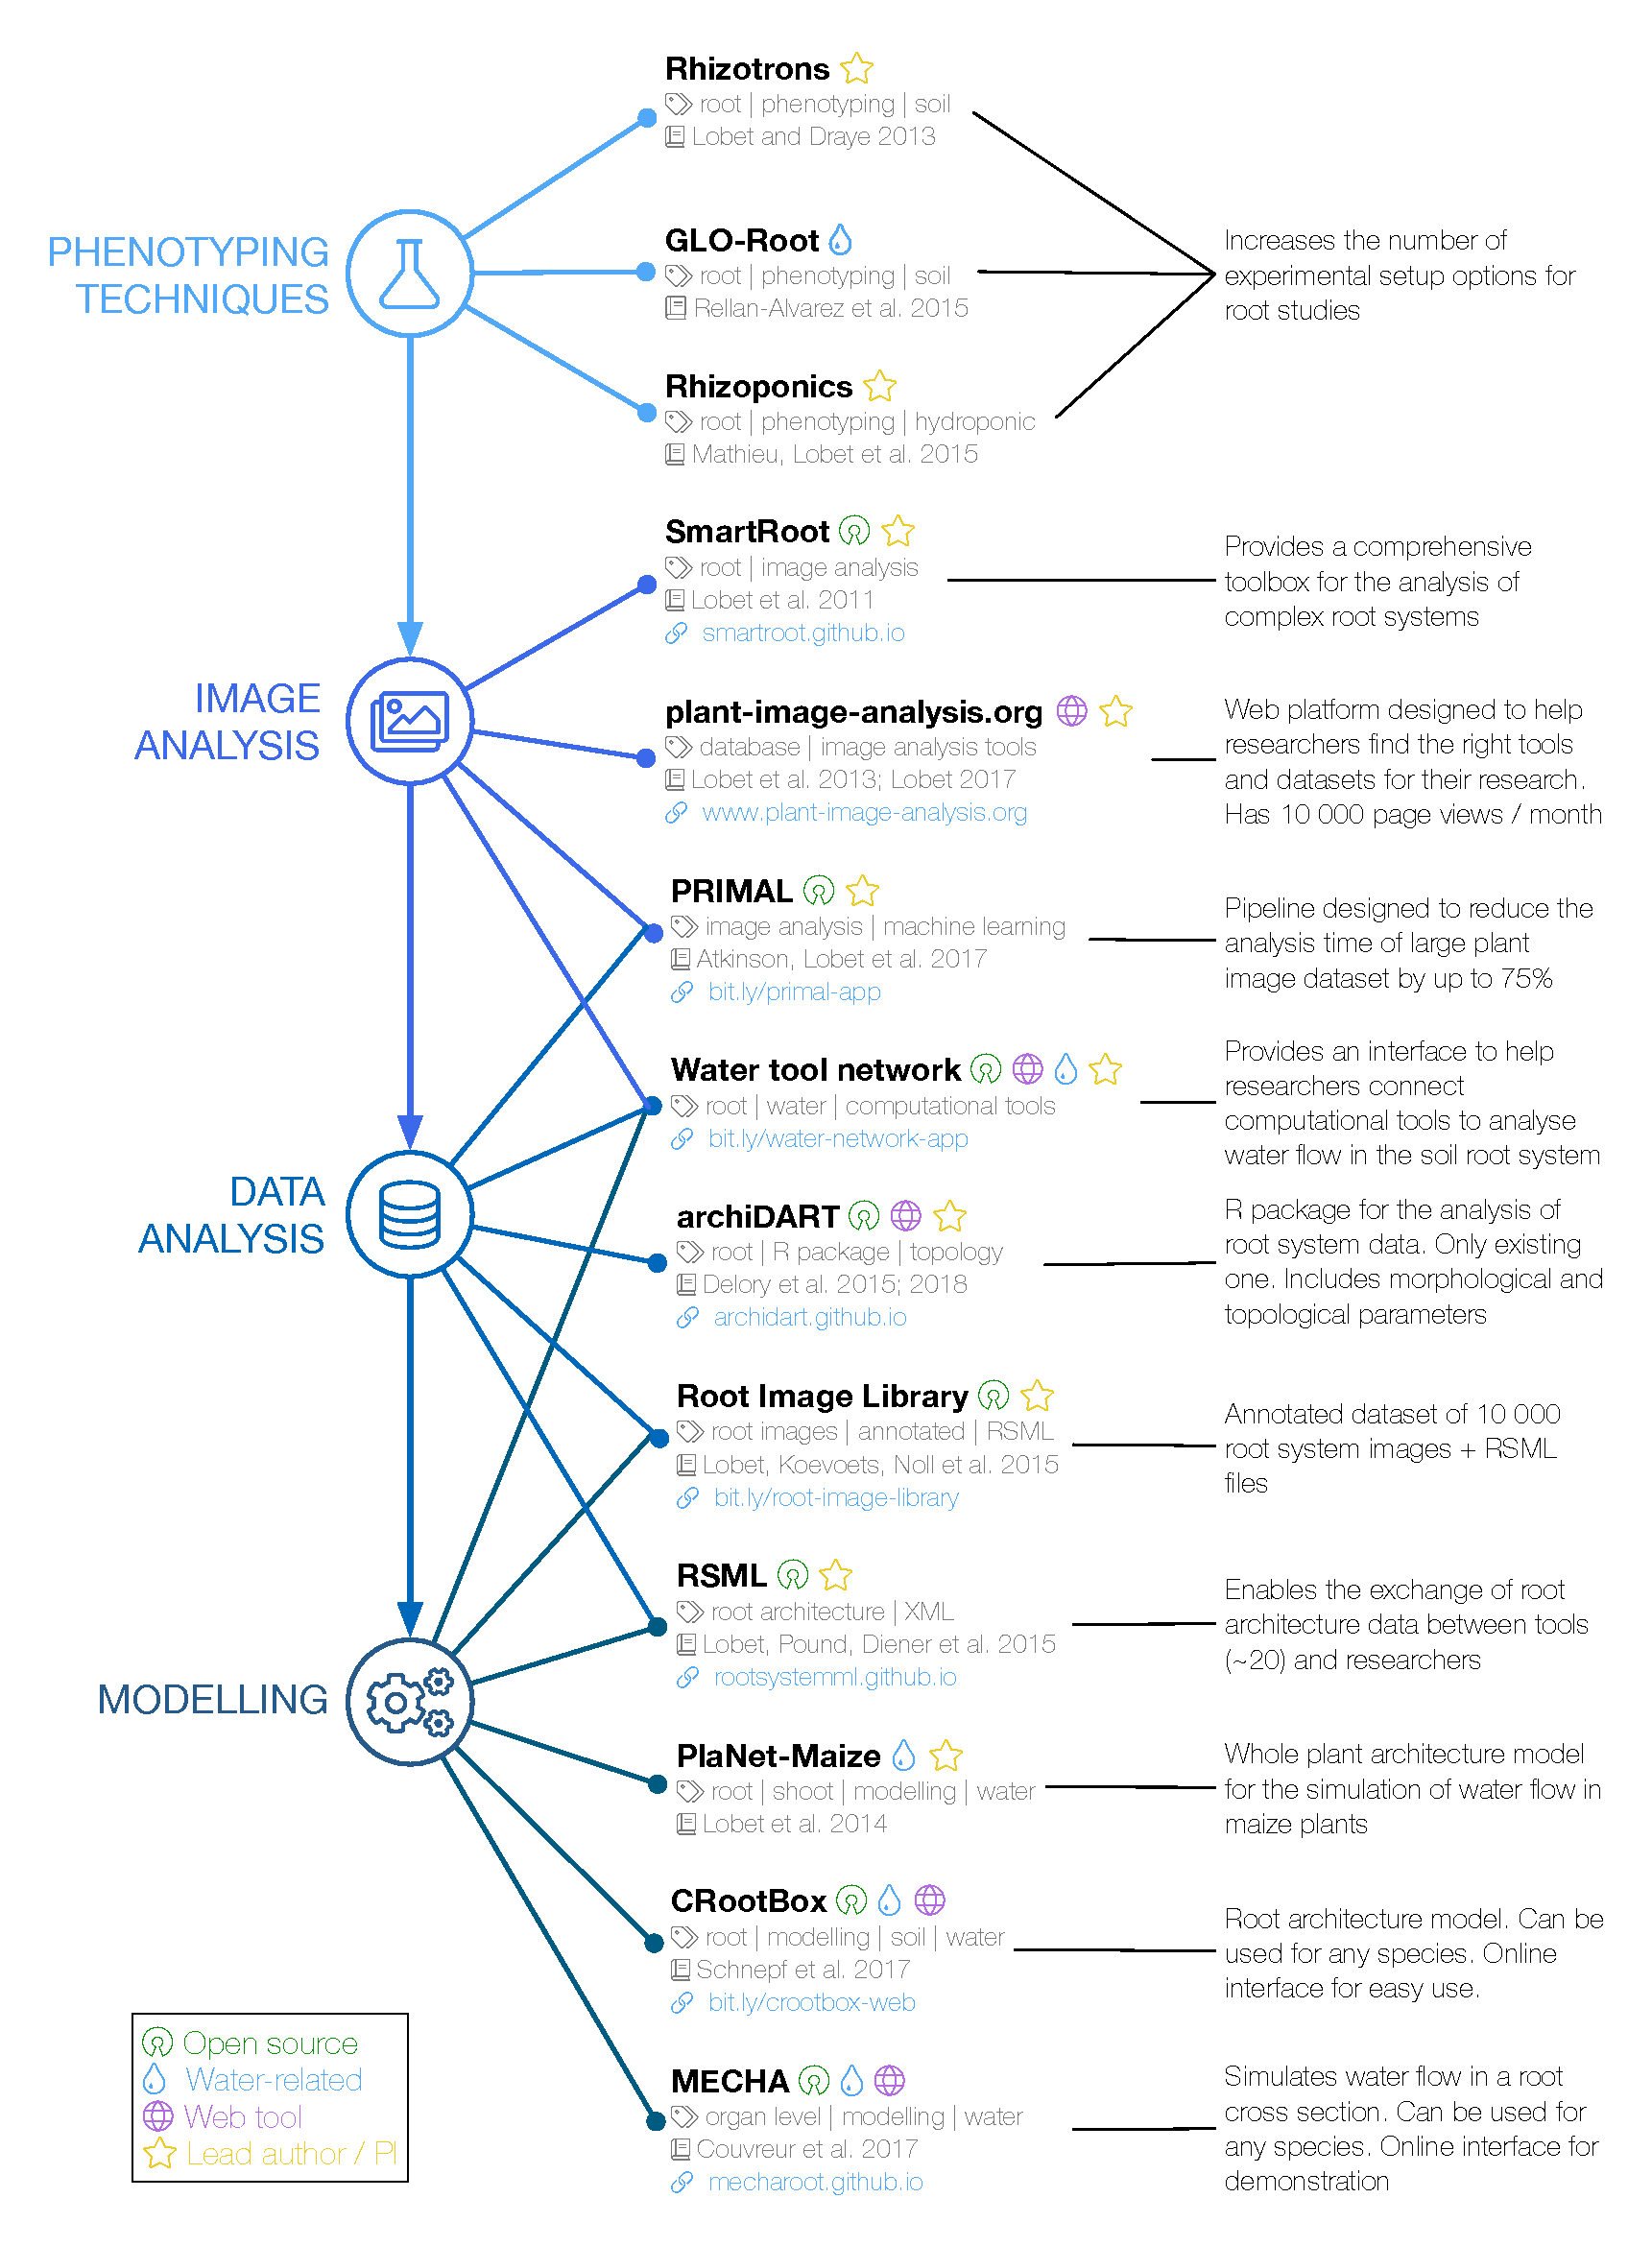
\includegraphics[width=1.3\linewidth]{work_overview}

\newpage
~
\vspace{0.05cm}

\section{Publications}

\vspace{0.5cm}
%\hline
\vspace{0.5cm}

\begin{tabular}{lp{0.8cm}|p{0.8cm}l}
    
    Peer-review publications: \textbf{26} & & &  Reviews performed: \textbf{58}\\
    Total number of citations: \textbf{597} & & & Invitations to conferences/workshops: \textbf{15}\\
    H-index: \textbf{12} & & & Organisation of conferences/workshops: \textbf{3}\\
   Guest editor: \textbf{GigaScience} & & & Academic editor: \textbf{Plant Direct}\\
\end{tabular}

\vspace{0.5cm}

\small{
    \begin{itemize}
    {\color{lightgray}
        \item Journal names were intentionally left blank.
        \item Link to all articles can be found on \href{http://www.guillaumelobet.be}{www.guillaumelobet.be}.
        \item Bibliometric data are coming from \href{http://www.dimensions.ai}{dimensions.ai} and \href{http://www.altmetric.com}{altmetric.com}.
        \item The Field Citation Ratio (FCR) indicates the relative citation performance of an article, when compared to similarly-aged articles in its subject area (1 = average).
        \item The Altmetric Score is an automatically calculated, weighted count of all of the attention a research output has received online. 
        }   
    \end{itemize}
}

\vspace{0.5cm}
%\hline
\vspace{0.5cm}

\begin{refsection}
\nocite{*}
\printbibliography[sorting=chronological, type=article, title={Pre-print articles\\}, keyword={preprint}, heading=subbibliography]
\end{refsection}


\begin{refsection}
\nocite{*}
\printbibliography[sorting=chronological, type=article, title={~\\Articles in peer-reviewed journals\\}, keyword={accepted}, heading=subbibliography]
\end{refsection}



%\begin{refsection}
%\nocite{*}
%\printbibliography[sorting=chronological, type=article, title={Articles in peer-reviewed journals - submitted}, keyword={submitted}, heading=subbibliography]
%\end{refsection}


%\printbibsection{incollection}{~\\Book chapters\\} 

%\printbibsection{thesis}{~\\PhD thesis\\}

%\begin{refsection}
%\nocite{*}
%\printbibliography[sorting=chronological, type=inproceedings, title={Articles in conference proceedings\\}, keyword={paper}, heading=subbibliography]
%\end{refsection}

\begin{refsection}
\nocite{*}
\printbibliography[sorting=chronological, type=inproceedings, title={~\\Invited presentations in international conferences\\}, keyword={invited}, heading=subbibliography]
\end{refsection}


\begin{refsection}
\nocite{*}
\printbibliography[sorting=chronological, type=inproceedings, title={~\\Presentations in international conferences\\}, keyword={spont}, heading=subbibliography]
\end{refsection}

%\printbibsection{misc}{Other publications} 








\end{document} 



